\chapter{Methodology}

In this chapter, we provide the detail procedures, steps that we have done in our research and how our results are obtained.\par\vspace{1em}


\section{Building pre-trained classifier model}
\begin{figure}
    \centering
    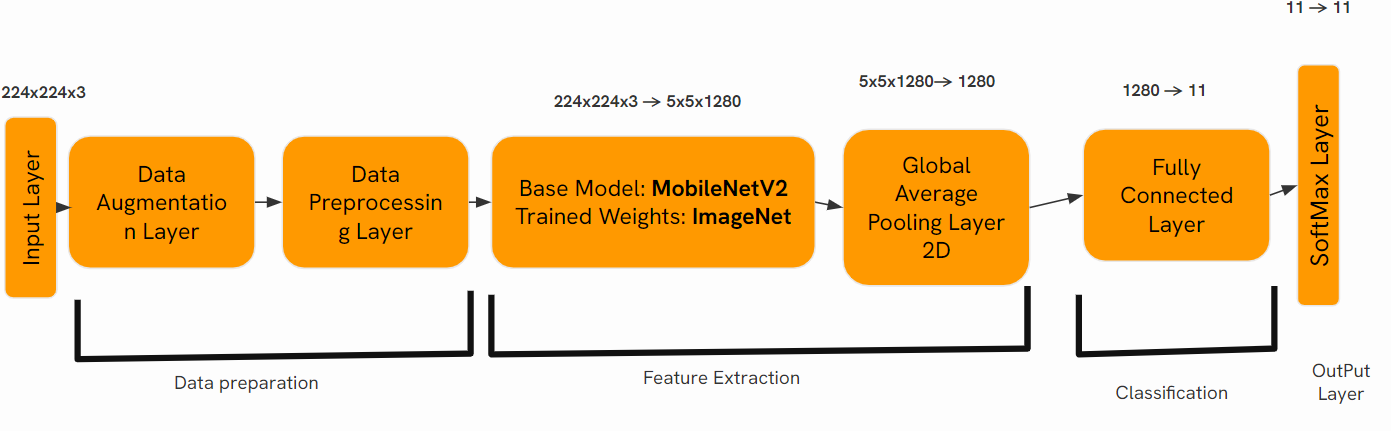
\includegraphics[width=1\linewidth]{graphics/chapter5/mobileNetV2 base model.png}
    \caption{MobileNetV2 Based Model}
    \label{fig:mobilenetv2-based-model}
\end{figure}

For building our model for performing transfer learning, we take the following steps.\\
We first build our data preprocessing pipeline which involves batching our images inorder to perform prediction, inference, prediction faster, resizing our image datasets to a desired shape that can be accepted by our model. After that, we load our pre-trained model by removing their top layers and added a single Fully Connected Layers (FCN) layer which have which have size equal to the number of classes that we want to perform classifications on.\par\vspace{1em}

For building our pre-trained classifier model, with MobileNetV2, refer fig\ref{fig:mobilenetv2-based-model} as base model, we first download the pretrained MobileNetV2 model with weights trained on \textbf{ImageNet datasets} and remove their top layers. Then, we add a \textbf{Global Average Pooling 2D Layer} on the top of the downloaded pretrained model to flatten the  7x7x1280 features map extracted by the base model, by taking the average of each 7 x 7 features map. Now, we add a single \textbf{FCN Layer} on top of Global Avg Pool 2D layer as the last layer. The number of neuron units in this FCN Layer is equal to 11 units as we are planning to classify 11 classes,\par\vspace{1em}

Similarly, we build other pretrained model using VGG-16 and Xception as base model, using the same procedures as above. The detailed description of each model layer is shown in fig \ref{fig:mob-vgg16-base-model} and \ref{fig:xception-base-model}.

\begin{figure}
     \begin{subfigure}{\linewidth}
        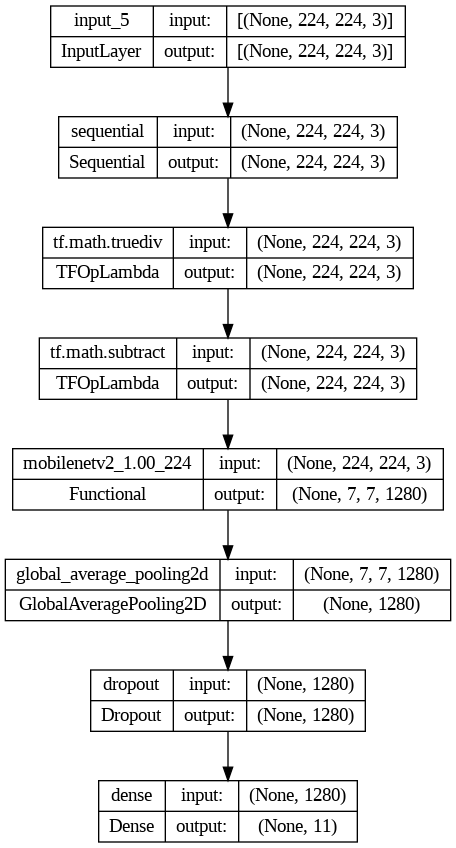
\includegraphics[width=.5\linewidth]{graphics/chapter5/mobilnetV2 based model graph.png}\hfill
        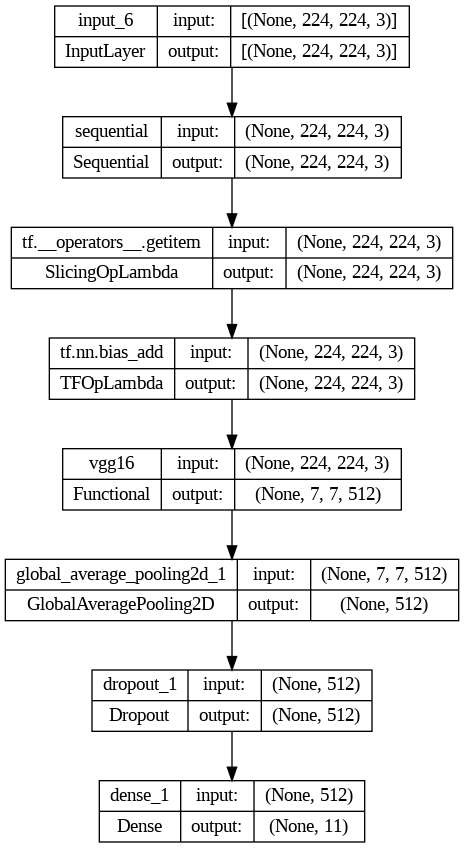
\includegraphics[width=.5\linewidth]{graphics//chapter5/vgg16 base model graph.png}\hfill
    \end{subfigure}    
    \caption{From left to right: MobilNetV2 Base Model, VGG-16 Base Model}
        \label{fig:mob-vgg16-base-model}    
\end{figure}

\begin{figure}
    \centering
    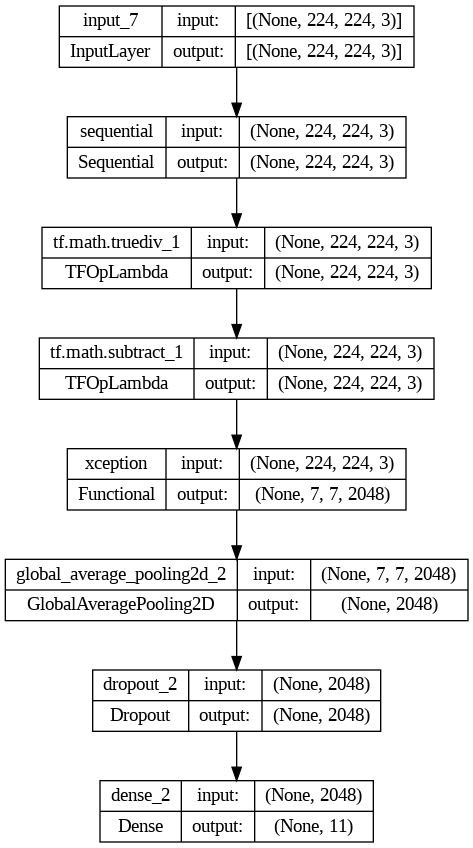
\includegraphics[height=\textheight]{graphics//chapter5/xception base model graph.png}
    \caption{Xception Base Model}
    \label{fig:xception-base-model}
\end{figure}


\section{Transfer Learning}\label{Transfer-learning-section}

\begin{figure}
    \centering
    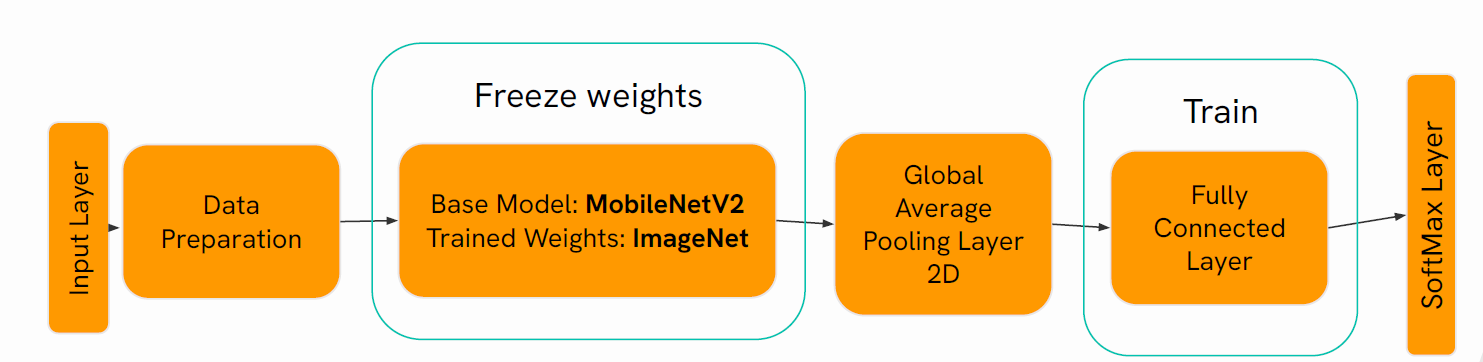
\includegraphics[width=\linewidth]{graphics//chapter5/transfer learning.png}
    \caption{Transfer Learning}
    \label{fig:transfer-learning}
\end{figure}

After building our MobileNetV2, VGG16, Xception base model, we start performing transfer learning and fine-tuning our models using our datasets. So, we first split our datasets on \textbf{80:10:10} ratios corresponding to training, testing and validation datasets size.\par\vspace{1em}

Then, we perform transfer learning by using the following approach, we freeze the weights of the entire base model, (i.e VGG16. Xception, MobileNetV2 part of our model), then we start training only the FCN layer of our models. Here, Freezing is a technique to prevents the weights in a given layer from being updated during training In this way, we trained our model without destroying the weights (knowledge) that it has learned previously (learned from \textbf{ImageNet datasets})\\
So, in transfer learning phase of the training, we just used our base model as a feature extractor and trained only the last top layer (FCN layer) that we added, to perform the classification task using the features extracted by the base model. 


\subsection{Model Training}

\begin{figure}
    \centering
    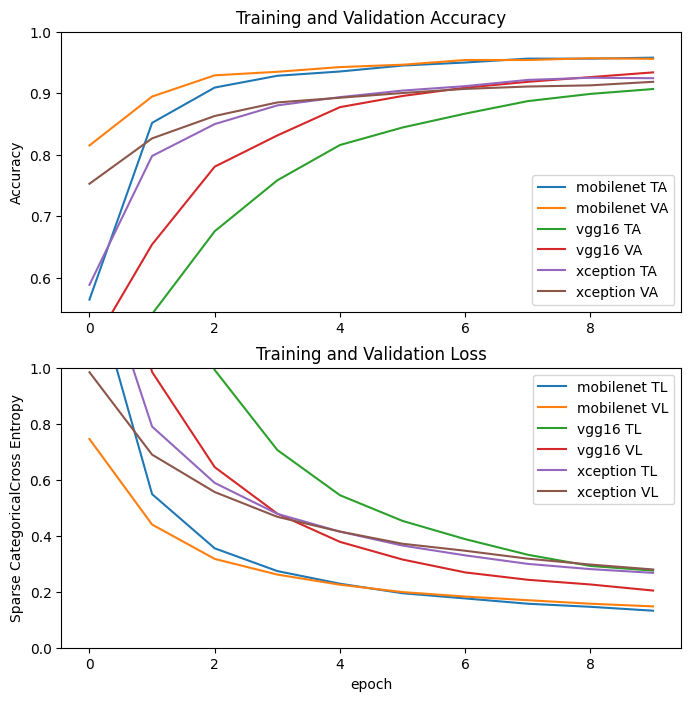
\includegraphics[width=1\linewidth]{graphics//chapter5/transfer learning training.png}
    \caption{Transfer Learning Training Graph}
    \label{fig:transfer-learning-training}
\end{figure}

\textbf{Parameters}:\par
\begin{itemize}
    \item \textbf{Epochs}: 10\par
    \item \textbf{Learning Rate}: $10^{-4}$\par
    \item \textbf{Loss Function}: Sparse Categorical Cross Entropy\par
    \item \textbf{Optimizer}: Adam\par
    \item \textbf{Metrics}: Accuracy
\end{itemize}


In the transfer learning phase, we observe that while training our model, MobileNetV2 base model converse fastest as compared to other models. So, we can say that MobileNetV2 is an excellent feature extractor as compared to the other 2 models that we used.


\section{Fine Tuning}
\textbf{Parameters}
\begin{itemize}
    \item \textbf{Epochs}: 10
    \item \textbf{Learning Rate}: $10^{-5}$
    \item \textbf{Loss Function}: Sparse Categorical Cross Entropy
    \item \textbf{Optimizer}: RMSProp
    \item \textbf{Metrics}: Accuracy
\end{itemize}


\begin{figure}
    \centering
    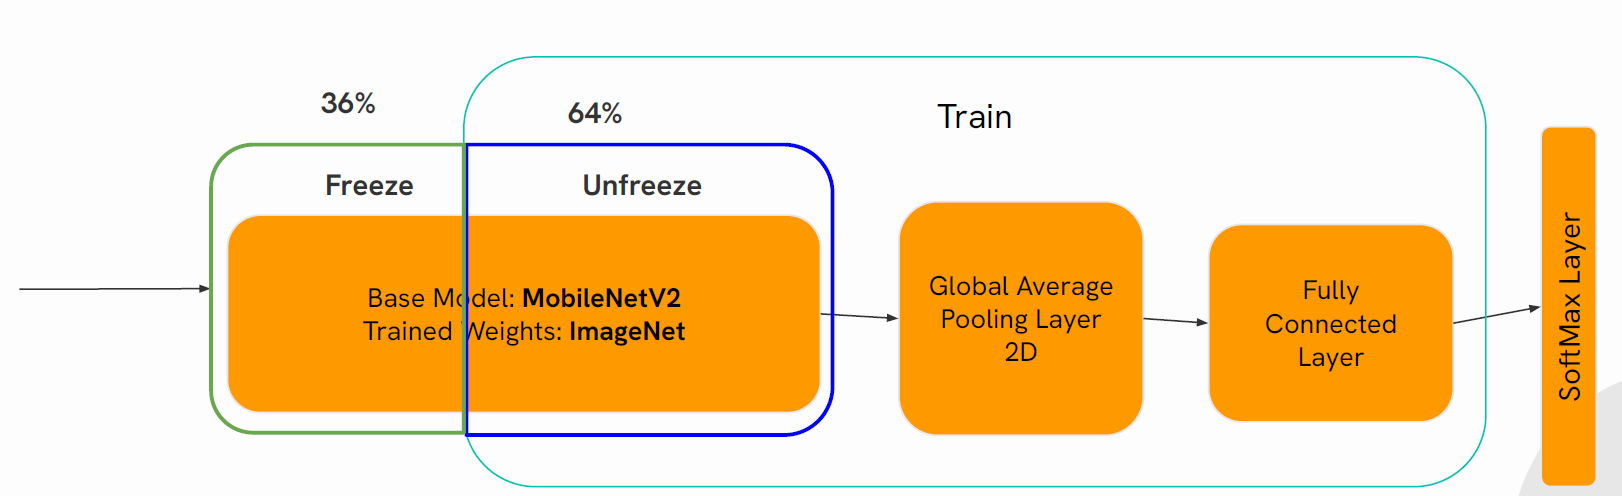
\includegraphics[width=1\linewidth]{graphics//chapter5/fine tuning.png}
    \caption{Fine Tuning}
    \label{fig:fine-tuning}
\end{figure}

We perform the fine-tuning phase of our model just after transfer learning phase, this phase of training is performed mainly to further increase the performance of our model on our particular training datasets.\\

In transfer learning, we were only training the top layers of our base model. The weights of the pre-trained network were not updated during training. One way to increase performance even further is to train (or "fine-tune") the weights of the top layers of the pre-trained model alongside the training of the classifier we added. The training process will force the weights to be tuned from generic feature maps to features associated specifically with the dataset.\par\vspace{1em}

Fine tuning of our model on Plant Village Datasets is perform in the following ways, we first unfreeze 64\% of the top layers of our base models and freeze the remaining 36\% of our model weights. Then, we again trained our model with our datasets with the unfreeze weights and the last FCN layer. \par\vspace{1em}

While fine tuning, we should try to fine-tune a small number of top layers rather than the whole base model layers. 
The reason why we unfreeze 64\% top layer of our base model and not unfreeze the entire base model weights is because in most convolutional networks, the higher up a layer is, the more specialized it is. The first few layers learn very simple and generic features that generalize to almost all types of images. As you go higher up, the features are increasingly more specific to the dataset on which the model was trained. The goal of fine-tuning is to adapt these specialized features to work with the new dataset, rather than overwrite the generic learning.\par\vspace{1em}

\subsection{Model Training}

\begin{figure}
    \centering
    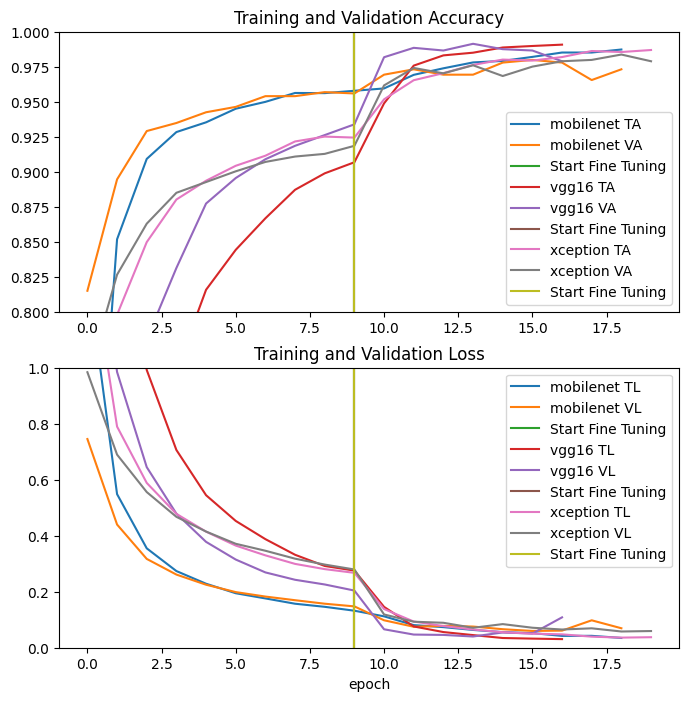
\includegraphics[width=1\linewidth]{graphics//chapter5/fine tuning training graph.png}
    \caption{Fine Tuning Training Graph}
    \label{fig:fine-tuning-training}
\end{figure}


During the fine-tuning phase of our model, we observe from the training curve graph, that the VGG-16 base model converges faster and outperforms other other models. So we can inferred that VGG-16 model can generalized well on specific datasets using its learned knowledge. \par\vspace{1em}

The success of VGG16 indicates that the pre-trained weights on ImageNet were highly beneficial and effectively transferable to the Plant Village dataset. VGG16’s architecture, with its deep layers, is adept at extracting intricate and hierarchical features, which are crucial for distinguishing between different plant diseases.\par\vspace{1em}

 The ability of VGG16 to effectively adapt pre-trained features to new data highlights the power of transfer learning and fine-tuning in achieving high accuracy and robust model performance. \par\vspace{1em}
 

\section{CNN10L ConvNet Model}
 We build our CNN10L Model using the specifications define in \ref{fig:CNN10L} and \ref{fig:cnn10l-detail-arch} 
 
\subsection{Model Training}
We trained our CNN10L model using \textbf{K Fold Cross Validation Method}. \\

So, in this technique, we first divide our dataset into train and test split in ratio of 90:10. Then, further divide our training set into K folds. After that, we perform K fold Cv Training of our model.
In the first phase (i.e. K = 1), we take the last fold as validation set and remaining as training set and perform training. Then in second K fold training phase (i.e. K = 2), we take the last second fold as validation set and remaining folds as training sets and again train our models. Similarly , we continue this process for K times taking $K^{th}$ fold as validation step. The steps for this training is shown clearly in the figure \ref{fig:k-fold}\par\vspace{1em}

\textbf{Parameters}:
\begin{itemize}
    \item \textbf{K }= 5 folds
    \item \textbf{Epochs:} 30 (with Early Stopping Condition)
    \item \textbf{Learning Rate:} $10^{-3}$
    \item \textbf{Loss Function:} Sparse Categorical Cross Entropy
    \item \textbf{Optimizer:} Adam
    \item \textbf{Metrics:} Accuracy
\end{itemize}

The training curve for our CNN10LL model for 5 K folds is shown in fig\ref{fig:cnn10l-fold1-3} and \ref{fig:cnn10l-fold4-5}\par\vspace{1em}

\begin{figure}
    \centering
    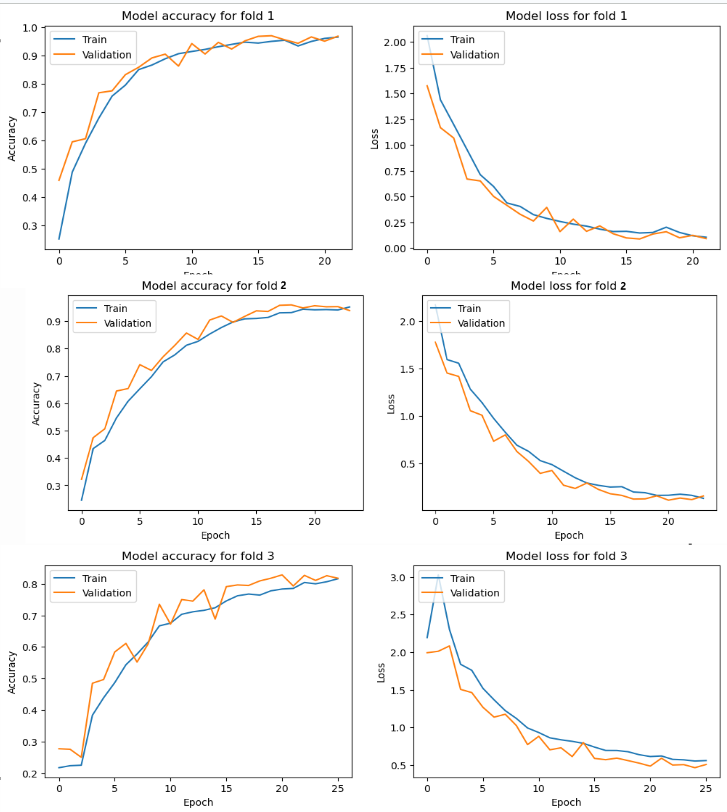
\includegraphics[width=1\linewidth]{graphics//chapter5/cnn10L training fold1-3.png}
    \caption{CNN10L Training for fold 1 to fold 3}
    \label{fig:cnn10l-fold1-3}
\end{figure}

\begin{figure}
    \centering
    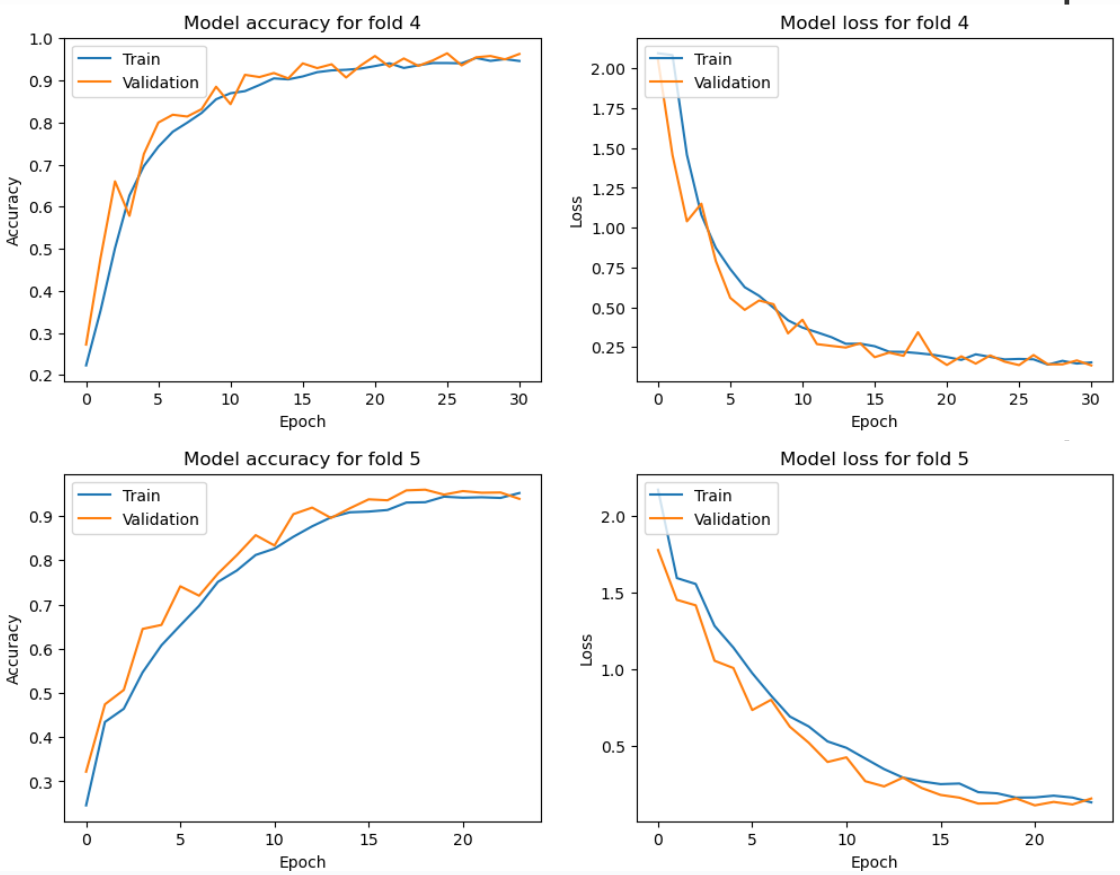
\includegraphics[width=1\linewidth]{graphics//chapter5/cnn10L training fold4-5.png}
    \caption{CNN10L Training for fold 4 to fold 5}
    \label{fig:cnn10l-fold4-5}
\end{figure}

\FloatBarrier


\section{Classical ML model as Classifier}

    \begin{figure}
        \centering
        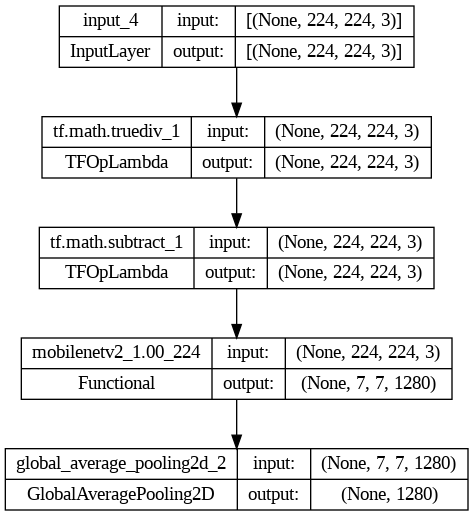
\includegraphics[width=0.75\linewidth]{graphics//chapter5/moboilenetv2 feature extractor.png}
        \caption{MobileNetV2 Feature Extractor used for training Classic ML Model}
        \label{fig:mobnetv2-feature-extractor}
    \end{figure}

\begin{figure}
    \centering
    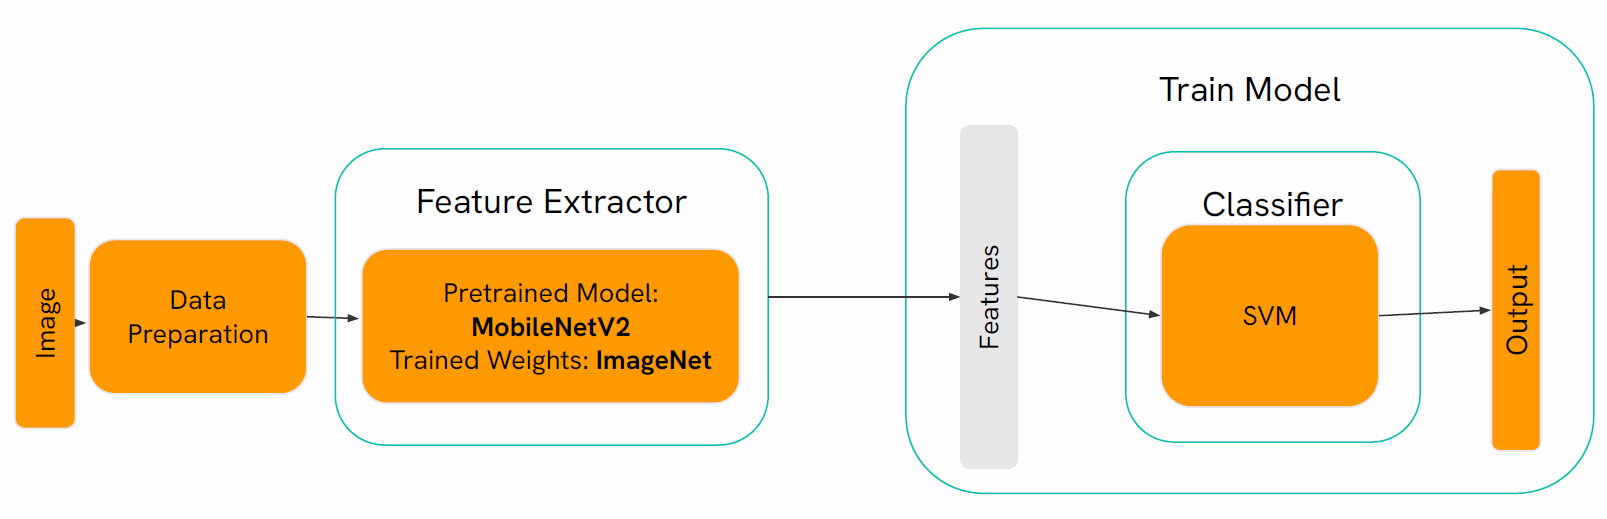
\includegraphics[width=1\linewidth]{graphics//chapter5/mobilenetV2 + SVM.png}
    \caption{MobilenetV2 + SVM}
    \label{fig:mobilenetv2-svm}
\end{figure}

\begin{figure}
    \centering
    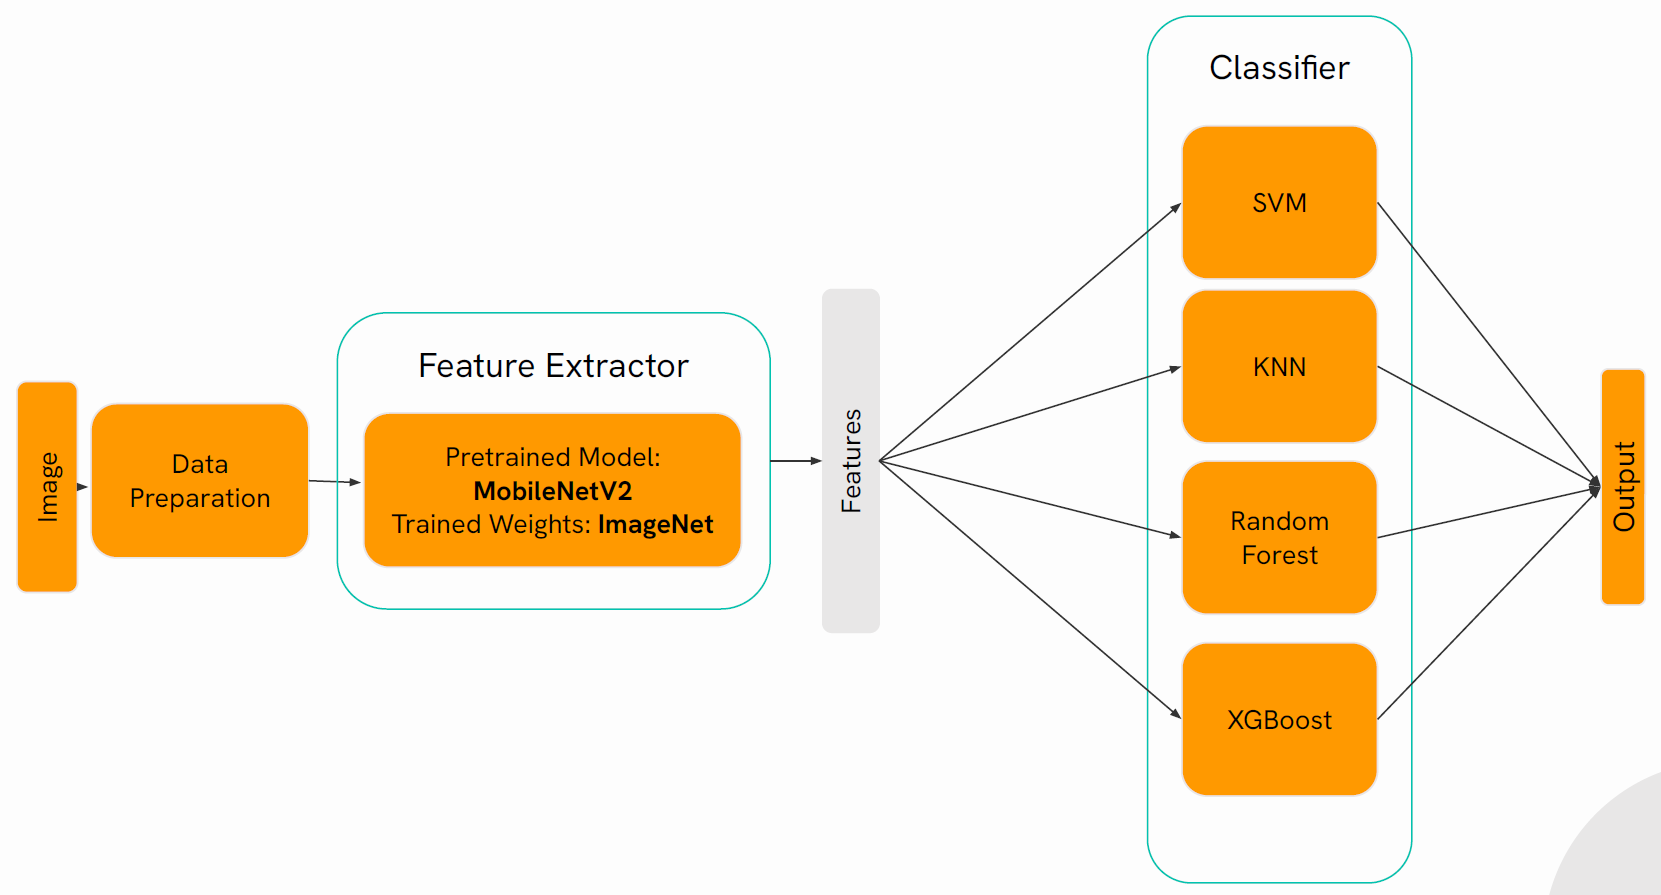
\includegraphics[width=1\linewidth]{graphics//chapter5/mobilentV2 + ML.png}
    \caption{MobileNetV2 + Traditional Classifier Models}
    \label{fig:mobilenetv2-all}
\end{figure}

    Since, classical ML classifier models such as SVM, KNN, Random forest, XBoost, etc cannot extract features directly from an image, we used a pretrained MobileNetV2 as a feature extractor for training these models.\par\vspace{1em}

    So, we first download a pretrained MobileNetV2 model (trained on \textbf{ImageNet}) and remove its top layer so that it gives the last feature maps as an output instead of the 1000 classes outputs. 
    Then, we input an image to this MobileNetV2, which give out a 7 x 7 x 1280 features map. we perform a global average pooling 2d on this output feature map to produce a 1280 features vector (7 x 7 x 1280 to 1 x 1 x 1280). \par\vspace{1em}
    In this way, we perform feature extraction for all the images in our dataset to convert it into 1280 feature vectors from an image of shape 256 x 256 x 3, then train our traditional classifier model on this extracted features
\FloatBarrier

